% Created 2019-02-20 Wed 13:07
% Intended LaTeX compiler: pdflatex
\documentclass[10pt]{beamer}
\usepackage[utf8]{inputenc}
\usepackage[T1]{fontenc}
\usepackage{graphicx}
\usepackage{grffile}
\usepackage{longtable}
\usepackage{wrapfig}
\usepackage{rotating}
\usepackage[normalem]{ulem}
\usepackage{amsmath}
\usepackage{textcomp}
\usepackage{amssymb}
\usepackage{capt-of}
\usepackage{hyperref}
\usepackage{minted}
\usepackage{tikz}
\definecolor{cwiRed}{HTML}{BF1238}
\definecolor{cwiBlue}{HTML}{0B5D7D}
\setbeamertemplate{footline}[text line]{%
\parbox{\linewidth}{\noindent\vspace*{2pt}\noindent\rule{\linewidth}{0.4pt}\\{\scriptsize\noindent\vspace*{7pt}\insertshortauthor\hfill\insertshorttitle\hfill\insertdate}}
}
\renewcommand*\footnoterule{}
\renewcommand{\vec}[1]{\mathbf{#1}}
\usepackage{lmodern}
\usetheme[progressbar=head]{metropolis}
\author{WISM454 Laboratory Class Scientific Computing, Jan-Willem Buurlage}
\date{\today}
\title{Advanced RNGs}
\hypersetup{
 pdfauthor={WISM454 Laboratory Class Scientific Computing, Jan-Willem Buurlage},
 pdftitle={Advanced RNGs},
 pdfkeywords={},
 pdfsubject={},
 pdfcreator={Emacs 26.1 (Org mode 9.1.14)}, 
 pdflang={English}}
\begin{document}

\maketitle

\section{RNG}
\label{sec:orgfe94112}
\begin{frame}[label={sec:org2736b12}]{What makes a good RNG?}
\begin{itemize}
\item \alert{Theoretical}
\begin{itemize}
\item Period
\item Uniformity
\end{itemize}
\item \alert{Empirical}
\begin{itemize}
\item Tasks using RNGs, check if output as expected
\item Predictability
\item Invertibility (security!)
\end{itemize}
\item \alert{Computational efficiency}
\item \alert{Space and time complexity}
\item \alert{Application specific requirements}
\end{itemize}
\end{frame}
\begin{frame}[label={sec:org19eb28c}]{Testing your RNG library}
\begin{itemize}
\item Basic theory can tell you about e.g. the period, uniformity of your RNG without
running it. Also: \alert{\(d-\text{dimensional}\) equidistribution}.
\item E.g., if LCRNG is used to generate points in \(d\)
dimensional space, confined to maximum of \(\sqrt[d]{d!m}\) parallel hyperplanes.
\((a, c, m) = (57, 53, 2^7 - 1)\), \textrightarrow \(~16\) lines
\begin{center}
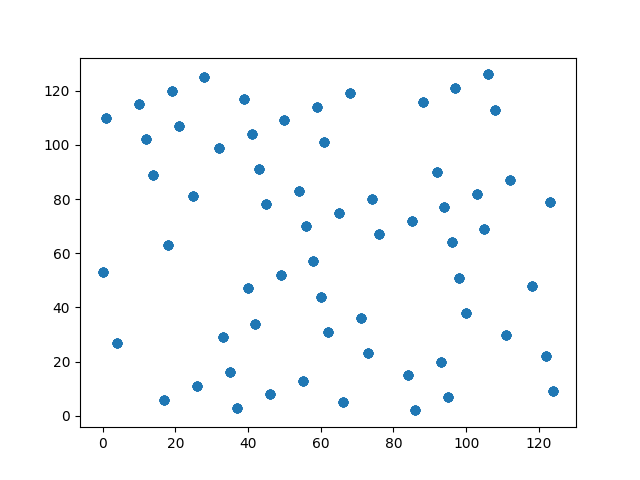
\includegraphics[height=0.65\textheight]{./hyperplanes.png}
\end{center}
\end{itemize}
\end{frame}
\begin{frame}[label={sec:org6ed358f}]{Software packages ('battery of tests')}
\begin{itemize}
\item There are software packages such as Diehard (1999) or
\alert{TestU01} (2007)\footnote{\url{http://simul.iro.umontreal.ca/testu01/tu01.html}} which
contain a collection of statistical tests for your RNGs.
\item TestU01 is a C library, can be made part of your code!
\item E.g. \alert{birthday paradox}, \alert{rank of random binary matrices}, \alert{play a game of
craps}, \alert{randomly place spheres in a box}, \ldots{} all follow a known
distribution.
\end{itemize}
\end{frame}
\begin{frame}[label={sec:org43878ce}]{Advanced RNGs}
Overview of topics today:

\begin{enumerate}
\item \alert{Xorshift}
\item Linear-feedback shift register
\item Mersenne twister
\end{enumerate}
\end{frame}
\begin{frame}[fragile,label={sec:org3e1bdca}]{Xorshift}
 \begin{minted}[frame=none,xleftmargin=\parindent]{cpp}
uint32_t xorshift(uint32_t x) {
    x ^= x << 13;
    x ^= x >> 17;
    x ^= x << 5;
    return x;
}
\end{minted}
\end{frame}
\begin{frame}[label={sec:orgf5d2d72}]{Xorshift\^{}[George Marsaglia (2003)]}
\begin{itemize}
\item Consider \(M = \{ 0, \ldots, m - 1 \}\), assume that our RNG is still of the form (for \(x_i \in M\)):
$$x_{i + 1} = f(x_i),$$
\item Generally, we want \(f\) to be be \alert{one-to-one}.
\item Usually not enough, since \(f = \text{id}\) is one-to-one but certainly not random.
\item Additionally require full period! (Although e.g. `f = (+1)` then still works)
\end{itemize}
\end{frame}
\begin{frame}[label={sec:org3594262}]{Linear transitions}
\begin{itemize}
\item Represent \(x_i \in M\) as binary vector:
$$\vec{x}^{(i)} = \begin{pmatrix}b_{0} \\ b_1 \\ \vdots \\ b_{n - 1} \end{pmatrix}$$
take \(f\) to be a linear function, i.e. given by \alert{transition matrix \(T\)}:
$$\vec{x}^{(i + 1)} = T \vec{x}^{(i)}.$$
\item \(T\) represents one-to-one function iff invertible
\item Limit to non-null vectors, i.e. full period consists of all \(m - 1\) non-zero integers in \(M\).
\end{itemize}
\end{frame}
\begin{frame}[label={sec:orgcdcab68}]{Exercise}
\begin{itemize}
\item \alert{\alert{Exercise:}} Prove that a non-singular \(T\) generates a non-zero sequence of full period for all non-zero seeds, if and only if the order of \(T\) is \(2^{n} - 1\) (in group of non-singular \(n \times n\) matrices)
\end{itemize}
\end{frame}
\begin{frame}[fragile,label={sec:orge11967a}]{Intermezzo: bitwise operations}
 \begin{itemize}
\item Bitwise operations are very efficient.
\begin{minted}[frame=none,xleftmargin=\parindent]{cpp}
uint8_t x = 0b00010010; // 18
uint8_t y = 0b01010010; // 82
\end{minted}
\item Shifts:
\begin{minted}[frame=none,xleftmargin=\parindent]{cpp}
x >> 2 // ~> 0b00000100
x << 2 // ~> 0b01001000
\end{minted}
\item Binary bitwise operations
\begin{minted}[frame=none,xleftmargin=\parindent]{cpp}
x ^ y // XOR ~> 0b01000000
x | y // OR  ~> 0b01010010
x & y // AND ~> 0b00010010
\end{minted}
\item We have that \texttt{1 << k} is equal to \(2^k\), and that XOR is addition modulo two
(i.e. addition in our vector space \((F_2)^n\))
\end{itemize}
\end{frame}
\begin{frame}[fragile,label={sec:orge8003ca}]{How to choose \(T\)}
 \begin{itemize}
\item Left shift \(L\) (i.e. \(Lx \equiv x \ll 1\)), right shift \(R\) (i.e. \(Rx \equiv x \gg 1\)):
$$L =
  \begin{pmatrix}
  0 & \ldots & \ldots & \ldots & 0 \\
  1 & \ddots & \ddots & \ddots & \vdots \\
  0 & 1 & \ddots & \ddots & \vdots \\
  \vdots & \ddots & \ddots & \ddots & \vdots \\
  0 & \ldots & 0 & 1 & 0 \\
  \end{pmatrix}, R =
  \begin{pmatrix}
      0 & 1 & 0 & \ldots & 0 \\
      \vdots & \ddots & 1      & \ddots & \vdots \\
      \vdots & \ddots & \ddots & \ddots & 0 \\
      \vdots & \ddots & \ddots & \ddots & 1 \\
      0 & \ldots & \ldots & \ldots      & 0
  \end{pmatrix}$$
\item Note that \(L^a x\), \(R^a x\) equal to \texttt{x << a} and \texttt{x >> a} respectively.
\item Clearly \(L\) and \(R\) singular.
\end{itemize}
\end{frame}

\begin{frame}[label={sec:org5aa53f4}]{The xorshift transition matrix}
\begin{itemize}
\item But: \(\text{Id} + L^a\) and \(\text{Id} + R^a\) non-singular! However, sadly
\begin{equation}
T = (\text{Id} + L^a)(\text{Id} + R^b)
\label{eq:try1}
\end{equation}
does not have the right order for any \(a, b\).
\item Instead choose 
\begin{equation}
T = (\text{Id} + L^a)(\text{Id} + R^b)(\text{Id} +
L^c)
\label{eq:try2}
\end{equation}
\item \alert{\alert{Exercise:}} Verify experimentally that for (\ref{eq:try1}) no \(a, b\) give \(T\) with required period for \(n = 32\)
\item \alert{\alert{Exercise:}}  Give all triples \((a, b, c)\) for which (\ref{eq:try2}) has full period
\end{itemize}
\end{frame}
\begin{frame}[fragile,label={sec:org64d9d12}]{Standard \texttt{xorshift}}
 \begin{itemize}
\item The standard Xorshift RNG engine has:
$$T = (Id + L^{5})(\text{Id} + R^{17})(\text{Id} + L^{13}).$$
\begin{minted}[frame=none,xleftmargin=\parindent]{cpp}
uint32_t xorshift(uint32_t x) {
    x ^= x << 13;
    x ^= x >> 17;
    x ^= x << 5;
    return x;
}
\end{minted}
\item There are versions with bigger state and/or more elaborate transition functions that outperform this basic version.
\end{itemize}
\end{frame}
\begin{frame}[label={sec:org6005dd1}]{Linear-feedback shift register}
\begin{itemize}
\item Xorshift is an example of a linear-feedback shift register
\end{itemize}

Let \(a \in \{0, 1\}\)
\begin{definition}
A (binary) sequence generated by a \emph{shift register} is one satisfying an $n$-term recursion:
$$a^{(i + n)} = f(a^{(i)}, \ldots, a^{(i + n - 1)}).$$
If $f$ is linear, we speak of a linear-feedback shift register.
\end{definition}
\end{frame}
\begin{frame}[fragile,label={sec:org559f6f9}]{Mersenne twister}
 \begin{itemize}
\item Another example of LFSR
\item period of \(2^{19937} - 1\).
\item slower, but \(k\text{-equidistributed}\)
\item very popular
\begin{minted}[frame=none,xleftmargin=\parindent]{cpp}
#include <random>

auto rng = std::mt19937(seed);
std::cout << rng() << "\n";

// PS:
class mt19937 { 
    uint32_t operator()() { ... }
};
\end{minted}
\end{itemize}
\end{frame}
\begin{frame}[label={sec:org15201d8}]{mt19937}
\begin{itemize}
\item From Wikipedia:
\end{itemize}
\begin{quote}
The Mersenne Twister is the default PRNG for the following software systems:
Microsoft Excel,[3] GAUSS,[4] GLib,[5] GNU Multiple Precision Arithmetic
Library,[6] GNU Octave,[7] GNU Scientific Library,[8] gretl,[9] IDL,[10]
Julia,[11] CMU Common Lisp,[12] Embeddable Common Lisp,[13] Steel Bank Common
Lisp,[14] Maple,[15] MATLAB,[16] Free Pascal,[17] PHP,[18] Python,[19][20]
R,[21] Ruby,[22] SageMath,[23] Scilab,[24] Stata.[25]
\end{quote}
\end{frame}



\begin{frame}[label={sec:orgef1999a}]{Expectations for your RNG library}
\begin{itemize}
\item Required
\begin{itemize}
\item Usable for randomized algorithms
\item LCRNG
\item Distributions: uniform int, uniform double, Gaussian
\end{itemize}
\item Optional but expected
\begin{itemize}
\item Xorshift
\item Tested with TestU01 / Diehard
\item Benchmarks (random numbers / second)
\end{itemize}
\item Extra credits
\begin{itemize}
\item Mersenne twister
\item Full test-suite based on e.g. TestU01
\item Personal statistical test
\item Other (personal?) engines
\item Extra distributions
\end{itemize}
\end{itemize}
\end{frame}

\section{C++}
\label{sec:orgdf64a5f}
\begin{frame}[fragile,label={sec:org1cf3c21}]{Polymorphism (I)}
 \begin{minted}[frame=none,xleftmargin=\parindent]{cpp}
class rng {
  public:
    virtual int next() = 0;
};

class lcrng : public rng {
    ...
    int next() override {
        return ...;
    }
    ...
};
\end{minted}

\begin{itemize}
\item Here, \texttt{rng} is the \alert{base} class and \texttt{lcrng} is the \alert{derived} class that
\alert{inherits} from the base class.
\end{itemize}
\end{frame}

\begin{frame}[fragile,label={sec:orgab12fb2}]{Polymorphism (II)}
 \begin{itemize}
\item An \alert{abstract class} is a class with at least one pure virtual function, like \texttt{rng} has:
\begin{minted}[frame=none,xleftmargin=\parindent]{cpp}
virtual int next() = 0;
\end{minted}
A \alert{non-abstract class}  is also called a \alert{concrete class}
\item Objects of an abstract type can not be manipulated by-value, because the
representation of an \texttt{rng} is unknown. They have to be manipulated using
references or pointers:
\begin{minted}[frame=none,xleftmargin=\parindent]{cpp}
void monte_carlo(rng& engine, ...) { ... }
\end{minted}
\item We call \texttt{monte\_carlo} with a \alert{concrete} RNG engine. At runtime, the function will call the \texttt{next} implementation of this \alert{concrete}
class\_ (e.g. \texttt{lcrng}).
\begin{minted}[frame=none,xleftmargin=\parindent]{cpp}
auto r = lcrng{14239, 5205, (1 << 30) - 1};
monte_carlo(r, ...)
\end{minted}
\end{itemize}
\end{frame}
\begin{frame}[fragile,label={sec:org15d2226}]{Polymorphism (III)}
 \begin{itemize}
\item Abstract classes allow us to leave the choice of e.g. RNG engine to the user,
and write our code independently of concrete realizations.
\begin{minted}[frame=none,xleftmargin=\parindent]{cpp}
class uniform_real_distribution {
  public:
    uniform_real_distribution(rng& engine)
        : engine_(engine) {}

    float sample() {
        return (float)engine.next() /
            (engine.max() - 1); 
    }

  private:
    rng& engine_;
}
\end{minted}
\end{itemize}
\end{frame}

\begin{frame}[fragile,label={sec:org08f53c3}]{Polymorphism (IV)}
 \begin{minted}[frame=none,xleftmargin=\parindent]{cpp}
class abstract {
  public:
    virtual void f() = 0;
};

class concrete : public abstract {
  public:
    void f() override {}
};

abstract a; // ERROR
concrete b; // fine

void f(abstract& a) {
    a.f(); // fine
}
\end{minted}
\end{frame}

\begin{frame}[fragile,label={sec:org3d1d0e9}]{Polymorphism (V)}
 \begin{minted}[frame=none,xleftmargin=\parindent]{cpp}
class abstract {
  public:
    virtual void f() = 0;

  protected:
    virtual void g() = 0;
    int x;

  private:
    void h() {}
    int y;
};
\end{minted}
\end{frame}

\begin{frame}[fragile,label={sec:orgb848068}]{Polymorphism (VI)}
 \begin{itemize}
\item Access specifier, e.g. \texttt{public}:
\end{itemize}
\begin{minted}[frame=none,xleftmargin=\parindent]{cpp}
class derived : public base ...
\end{minted}
\begin{itemize}
\item \texttt{private} members of \texttt{base} are never visible to \texttt{derived}.
\item access specifier specifies maximum visibility of inherited members
\end{itemize}
\begin{itemize}
\item E.g.
\texttt{class derived : protected base} would make \texttt{public} and \texttt{protected}
members of \texttt{base}, \texttt{protected} members of \texttt{derived}.
\item For purposes other than inheriting, \texttt{protected} is like \texttt{private}.
\end{itemize}
\end{frame}

\begin{frame}[fragile,label={sec:org968fed3}]{RAII}
 \begin{minted}[frame=none,xleftmargin=\parindent]{cpp}
class object {
  public:
    object() { std::cout << "Constructor\n"; }
    ~object() { std::cout << "Deconstructor\n"; }
};

void f() {
    object o;
}

f();

auto o = new object;
delete o;
\end{minted}
\end{frame}

\begin{frame}[fragile,label={sec:org258f839}]{Heap storage}
 \begin{itemize}
\item User defined types with heap storage
\begin{minted}[frame=none,xleftmargin=\parindent]{cpp}
class rng_with_big_state : public rng {
  public:
    rng_with_big_state() {
        state_  = new State;
    }
    ~rng_with_big_state() {
        if (state_) { delete state_; }
    }
  private:
    State* state_;
};
\end{minted}
\item Hidden \texttt{new} and \texttt{delete}, safer user code:
\begin{minted}[frame=none,xleftmargin=\parindent]{cpp}
void monte_carlo() {
    auto r = rng_with_big_state(); // or:
    rng_with_big_state r; // same thing
}
\end{minted}
\end{itemize}
\end{frame}
\begin{frame}[label={sec:orgd67584e}]{Polymorphism and RAII}
\begin{itemize}
\item \alert{Derived classes} inherit from \alert{base classes}.
\item \alert{Abstract classes} versus \alert{concrete classes}.
\item Access specifiers
\item RAII allows automatic resource management based on scopes
\item These are very important concepts, crucial to understanding how to develop
quality C++ software. Spend some time familiarizing yourself with these
concepts!
\item \alert{\alert{Any questions/comments on polymorphism and RAII?}}
\end{itemize}
\end{frame}
\begin{frame}[fragile,label={sec:org3b4012f}]{Templates}
 \begin{itemize}
\item Up to now we have discussed runtime polymorphism (also \alert{virtual dispatch}). Templates are 'compile time polymorphism' (\alert{static dispatch}).
\begin{minted}[frame=none,xleftmargin=\parindent]{cpp}
struct distribution_u32 {
    uint32_t sample(rng& engine);
};
struct distribution_i32 {
    int32_t sample(rng& engine);
};
struct distribution_u64 {
    uint64_t sample(rng& engine);
};
struct distribution_f32 {
    float sample(rng& engine);
};
\end{minted}
\item \ldots{} there must be an easier way
\end{itemize}
\end{frame}

\begin{frame}[fragile,label={sec:org3218ec4}]{Enter templates!}
 \begin{minted}[frame=none,xleftmargin=\parindent]{cpp}
template <typename T> 
struct distribution {
    virtual T sample(rng& engine) = 0;
};

struct normal_distribution : distribution<float> {
    float sample(rng& engine) override {
        return ...;
    }
};
\end{minted}
\end{frame}

\begin{frame}[fragile,label={sec:org9ed70db}]{Fancy tricks!}
 \begin{minted}[frame=none,xleftmargin=\parindent]{cpp}
template <typename T,
typename std::enable_if_t<std::is_floating_point_v<T>>>
struct normal_distribution : distribution<T> {
    normal_distribution(T mean, T stddev) { ... }

    T sample(rng& engine) override {
        return ...;
    }
};
\end{minted}
\end{frame}
\begin{frame}[fragile,label={sec:org50b0207}]{Other examples}
 \begin{itemize}
\item Functions can be templates too, compile time values also allowed as \alert{template arguments}.
\begin{minted}[frame=none,xleftmargin=\parindent]{cpp}
template <int D, typename T>
std::vector<std::array<T, D>> generate_points(
    int count, distribution<T>& f) {
    return ...;
}
\end{minted}
\item Many STL types are templates. We will revisit templates when we discuss the standard library next week!
\end{itemize}
\end{frame}
\section{Tutorial}
\label{sec:org0c64ab9}
\begin{frame}[fragile,label={sec:orgbd49939}]{Exercises}
 \begin{itemize}
\item I have compiled all the exercises in a file \texttt{exercises.pdf}. See the GitHub
page.
\item Implement LCRNG, Xorshift engines
\item Implement distributions:
\begin{itemize}
\item Uniform
\item Gaussian (with rejection)
\item Something with inversion
\end{itemize}
\item Write function to randomly permute an array
\item Statistically test your generators
\end{itemize}
\end{frame}
\end{document}